\documentclass{beamer}
\usepackage[croatian]{babel}
\usepackage[utf8]{inputenc}
\usepackage{graphicx}
\usepackage{hyperref}
\usepackage{natbib}
\usepackage{bibentry}

\usetheme{PaloAlto}
\usecolortheme{fly}

\title{\textbf{Git Hooks}}



\subtitle{\textit{autori:} \newline 
Matej Anić\newline
Karlo Veršić\newline
Ani Perušić
}


\begin{document}
	\frame {
		\titlepage
		
	}
	\frame{
		\begin{figure}
			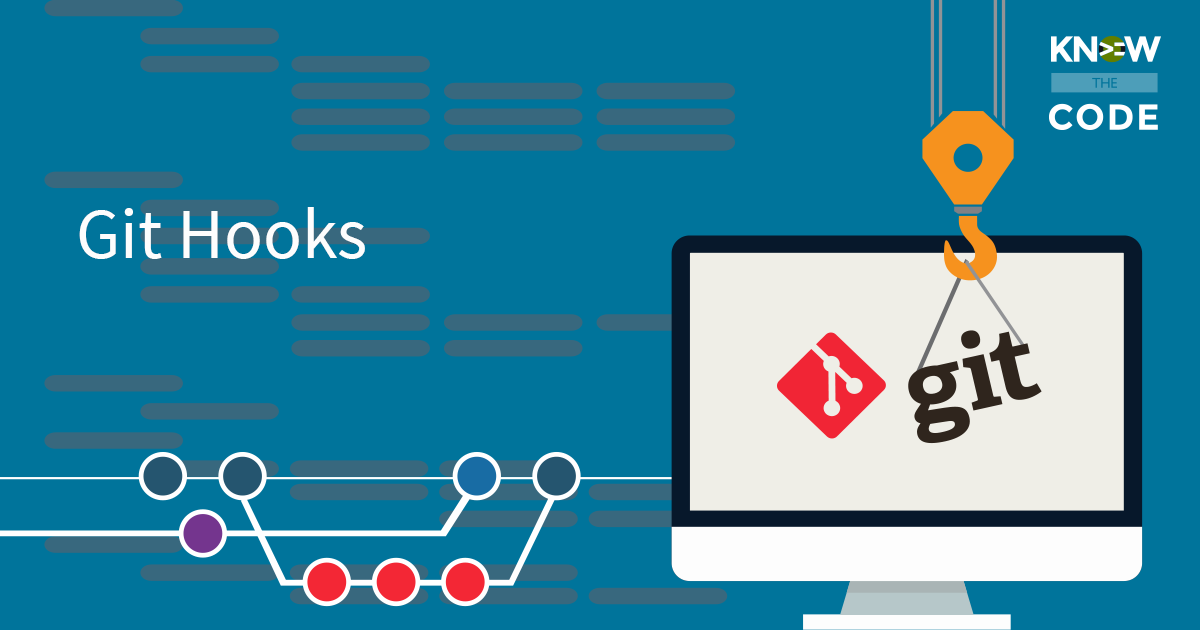
\includegraphics[scale=0.25]{pic3.png}
		\end{figure}
	}
	\frame {
		\frametitle{Što su Git hooks?}

		\textbf{Git Hooks} su skripte koje Git izvršava prije ili nakon događaja kao što su: \textit{commit, push} i \textit{receive}.
		\newline
		\newline
		Skripte se personaliziraju i prilagođavaju prema potrebi korisnika (npr. pri optimizaciji razvojnog toka, mijenjanju okruženja, te poticanju korištenja 		  			\textit{commit} funkcije).
		
	}
	\frame{
		\frametitle{\textit{Primjeri Git Hooks skripti:}}

		
		\underline{pre-commit}: (provjera poruke uz commit)\newline
		\underline{post-commit}: (slanje obavijesti o novome commitu)
		
	}
	\frame{
		\begin{figure}
			\caption{\textit{primjer: pre-commit}}
			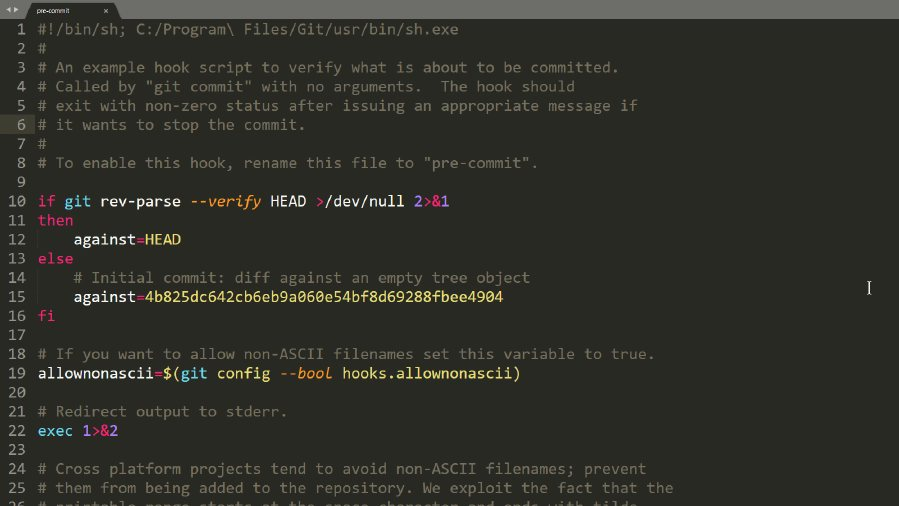
\includegraphics[scale=0.3]{pic2.jpg}
		\end{figure}
	}
	\frame{
		\frametitle{Kako funkcioniraju?}
		Svaki Git repozitorij ima \textit{.git/hooks} direktorij koji sadrži standardne Git Hooks skripte.\newline
		Slobodno se mogu izmjenjivati ili ažurirati, a Git će ih automatski izvršiti kada budu potrebne.
	}
	\frame{
		\frametitle{Svrha}
		Mogu napraviti različite zadatke.\newline
		Povećavaju produktivnost programera jer mu daju nove mogućnosti.\newline
		\newline
		Po potrebi možemo stvoriti i naše.
	}
	\frame{
		\frametitle{Najčešće svrhe}
		\begin{itemize}
            \item Uređivanje okoliša commitova, obavještavnje suradnika
            \item Optimizacija workflowa
            \item Uređivnje okoliša za izvršavanje koda
        \end{itemize}
        Može se koristiti i za skoro bilo koju drugu svrhu,\newline 
        zbog lakoće uređivanja skripti pa je teško izdvojiti najčešće svrhe.
        
        
	}
	\frame{
		\frametitle{Jezici za skripte}
		Ugrađene skripte su skoro uvijek PERL ili shell skripte,\newline
		ali se mogu koristiti i drugi programski jezici.\newline
		U prvoj liniji trebamo samo definirati kako će se skripta izvoditi.\newline
		Npr. na kraju reda dodati "python" ako kodiramo u Phytonu.
		}
	\frame{
		\frametitle{Problemi}
		Sadržaj .git direktorija se ne dijeli kad se dijele druge datoteke u repozitoriju.\newline
		Trebaju se dijeliti kopiranjem.\newline
		Mogu se i dijeliti stvaranjem direktorija predloška (Template Directory).\newline
		Sve datoteke iz tog direktorija se stavljaju u .git direktorij\newline
		prilikom korištenja "git init" i "git clone" naredbi.
	}
	\frame{
		\frametitle{Lokalni hooks}
		Odnose se samo na repozitorij u kojem djeluju.\newline
		Npr. pre-commit, post-commit
	}
	\frame{
		\frametitle{Server-side hooks}
		Nalaze se u centralnom ili javnom repozitoriju.\newline
		Mogu služiti za npr. odbijanje commitova.\newline
		Npr. pre-recive, update, post-recive.
	}
	\frame{
		\frametitle{Literatura}
		\url{https://githooks.com/}
		\url{https://www.atlassian.com/git/tutorials/git-hooks}
		

		
		\bibliographystyle{plain}
		\bibliography{bibfile}
	}
\end{document}